\documentclass[10pt]{article}
\usepackage[margin=0.58in]{geometry}
\usepackage{booktabs,enumitem,fancyhdr,graphicx,listings,tabularx,tikz,titlesec}
\graphicspath{{docs/lessons/assets/}{../assets/}}
\usetikzlibrary{arrows.meta,decorations.pathmorphing,positioning,shapes.geometric}
\usepackage[hidelinks]{hyperref}
\hypersetup{pdftitle={ADK Lesson 055: Constraint and Clue Model},
 pdfauthor={Kevin Shanahan},
 pdfsubject={Fixed-capacity clue rules, copied provenance, deterministic evaluation, and E0 replay},
 pdflang={en-US}}
\pagestyle{fancy}\fancyhf{}
\lhead{\textsc{ADK Lesson 055}}\rhead{Constraint and Clue Model}
\cfoot{\thepage}\setlength{\headheight}{14pt}
\setlength{\parindent}{0pt}\setlength{\parskip}{2.5pt}
\setlist{nosep,leftmargin=1.45em}
\titleformat{\section}{\Large\bfseries}{\thesection}{0.5em}{}
\newcommand{\lessonbox}[1]{\begin{center}\fbox{\parbox{0.92\linewidth}{#1}}\end{center}}
\newcommand{\blankline}{\rule{0.72in}{0.4pt}}
\newcommand{\longblank}{\rule{1.25in}{0.4pt}}
\tikzset{
 pencil line/.style={
  draw=black,thick,line cap=round,line join=round,
  dash pattern=on 3.6pt off .18pt on 1.1pt off .12pt,opacity=.88},
 pencil box/.style={
  rectangle,rounded corners=1.5pt,minimum height=7mm,align=center,
  fill=black!3,pencil line,inner sep=3pt},
 pencil arrow/.style={pencil line,-{Latex[length=2.2mm]}},
 faint pencil/.style={
  draw=black!60,line cap=round,line join=round,
  dash pattern=on 2.7pt off .15pt on .8pt off .1pt,opacity=.78}
}
\lstset{
 basicstyle=\ttfamily\footnotesize,
 columns=fullflexible,
 breaklines=true,
 frame=single,
 rulecolor=\color{black},
 showstringspaces=false
}

\begin{document}
\small
\begin{center}
 {\Huge\bfseries Constraint and Clue Model}\\[3pt]
 {\Large Turn copied clue cards into a deterministic rule result}\\[7pt]
 \fbox{\textbf{E0 COPIED POLICY REPLAY --- ZERO HARDWARE}}
\end{center}
\begin{tabularx}{\linewidth}{@{}>{\bfseries}l X >{\bfseries}l X@{}}
Lesson & 055 --- component & Time & 150--210 minutes\\
Prerequisite & copied evidence and modular time & Board & compile-only Mega replay\\
Capacity & 12 clues, 12 rules & Observation & named memory result cells\\
\end{tabularx}

\lessonbox{\textbf{Responsibility.} \texttt{ClueConstraintModel} owns one
fixed rule graph and copied clue evidence. It validates source identity,
sequence, time, quality, and prerequisites before publishing masks and a
model disposition. It owns no endpoint, pin, clock, display, storage medium,
latch, lamp, lock, or physical room.}

\section{Begin with an evidence wall, not a magic answer}
Each clue has one dense ID from zero, one fixed source identity, and one
matching slot and mask bit. An update is an entire envelope: selected slots
must contain matching clue IDs, while unselected slots must be canonical
zero. A malformed slot rejects the whole update rather than mixing old and
new evidence.

\begin{center}
% ADK visual: pencil
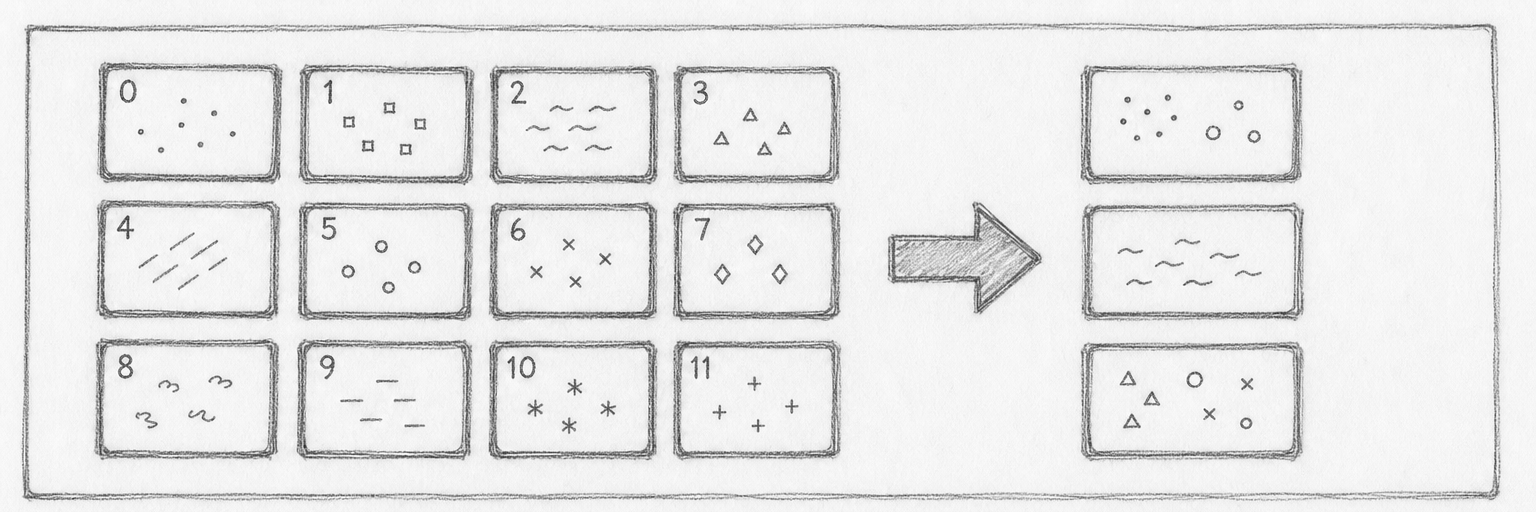
\includegraphics[width=0.94\linewidth,height=1.72in,keepaspectratio]
 {055-clue-wall-pencil.png}

\small\textit{Alternative text: a visibly hand-drawn wall of twelve clue
cards records source, sequence, time, and quality. One sketched arrow leads
to satisfied and blocked rule masks plus a model disposition.}
\end{center}

This is a conceptual memory drawing, not a circuit layout or formal
schematic. The ``wall'' is an array in memory. The named observation place
for this E0 lesson is \texttt{evidenceWallCells[]} in the canonical sketch.

\section{Build a directed acyclic rule graph}
A rule contains at most four terms and four prerequisite rule IDs. A term
compares one clue category with \texttt{Equals} or \texttt{NotEquals}.
Prerequisites are evaluated first. IDs are dense and unique; duplicate terms,
duplicate prerequisites, self-edges, out-of-range IDs, noncanonical unused
fields, and any cycle make initialization fail.

\begin{center}
% ADK visual: pencil
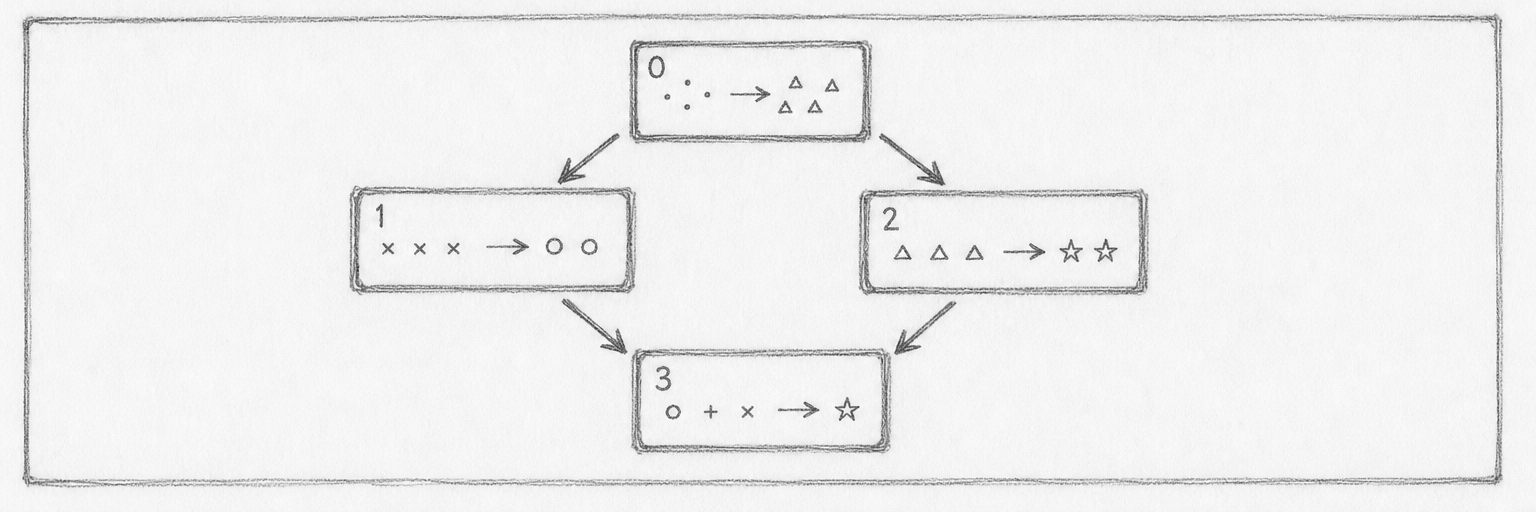
\includegraphics[width=0.88\linewidth,height=2.15in,keepaspectratio]
 {055-rule-dag-pencil.png}

\small\textit{Alternative text: a graphite diamond graph has rule zero
feeding rules one and two, which both feed rule three. Rule three cannot be
satisfied before both prerequisites.}
\end{center}

The model compiles this graph to a stable iterative order during
\texttt{initialize()}. It uses no recursion, allocation, callback, hidden
clock, or container iteration order.

\section{Predict evaluation precedence}
For a structurally valid envelope, evidence is classified before term
matching. Source, timing, invalid quality, or failing status is invalid;
stale precedes contradictory; contradictory precedes missing. A category
mismatch is ordinary unsatisfied evidence. For each rule, a failed
prerequisite precedes its terms.

\begin{tabularx}{\linewidth}{@{}l X X@{}}
\toprule
Observed condition & Rule prediction & Model consequence\\
\midrule
qualified, fresh, matching category & term may satisfy & continue through DAG\\
qualified, fresh, different category & \texttt{Unsatisfied} & incomplete\\
required clue absent & \texttt{MissingEvidence} & incomplete\\
invalid source, time, quality, or status & \texttt{InvalidEvidence} &
invalid evidence\\
older than inclusive age limit & \texttt{StaleEvidence} & stale evidence\\
explicit contradiction & \texttt{ContradictoryEvidence} & contradiction\\
failed prerequisite & \texttt{BlockedByPrerequisite} & blocked mask bit set\\
all rules satisfied & \texttt{Satisfied} & solved\\
\bottomrule
\end{tabularx}

\section{Keep provenance attached to every cell}
An accepted clue retains category, quality, exact expected source ID,
configuration revision, session epoch, source sequence, observation time,
and complete status. A changed value at the same sequence is invalid. Forward
sequence including rollover is accepted; regression and exact-half-range
ambiguity reject. Update-array order never supplies precedence.

\begin{center}
% ADK visual: pencil
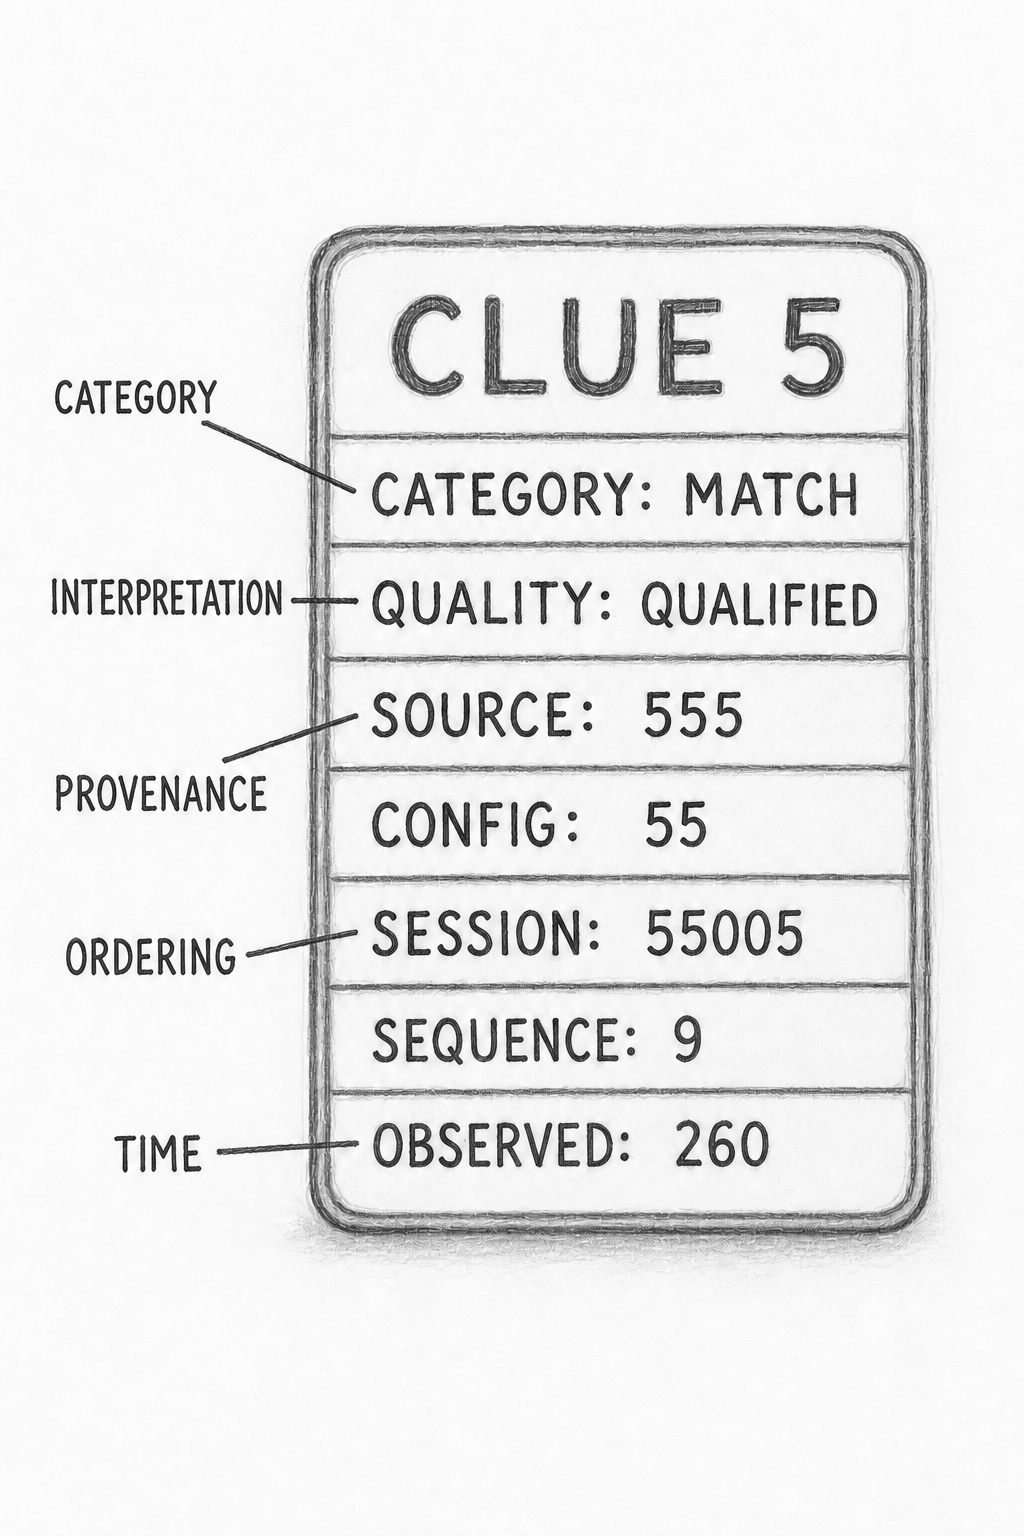
\includegraphics[width=0.72\linewidth,height=3.55in,keepaspectratio]
 {055-provenance-pencil.png}

\small\textit{Alternative text: a sketched clue-five record lists category,
quality, source identity, configuration, session, sequence, and time. Pencil
leader lines label category, interpretation, provenance, ordering, and time
as inseparable evidence.}
\end{center}

\newpage
\section{Treat freshness as an inclusive interval}
The caller supplies \texttt{now}; the model never reads wall time. With
\texttt{maximumEvidenceAge = 100}, evidence observed at 120 is fresh through
220 and stale at 221. A future timestamp, regression, duration at or above
the unsigned half range, or ambiguous order rejects atomically.

\begin{center}
% ADK visual: pencil
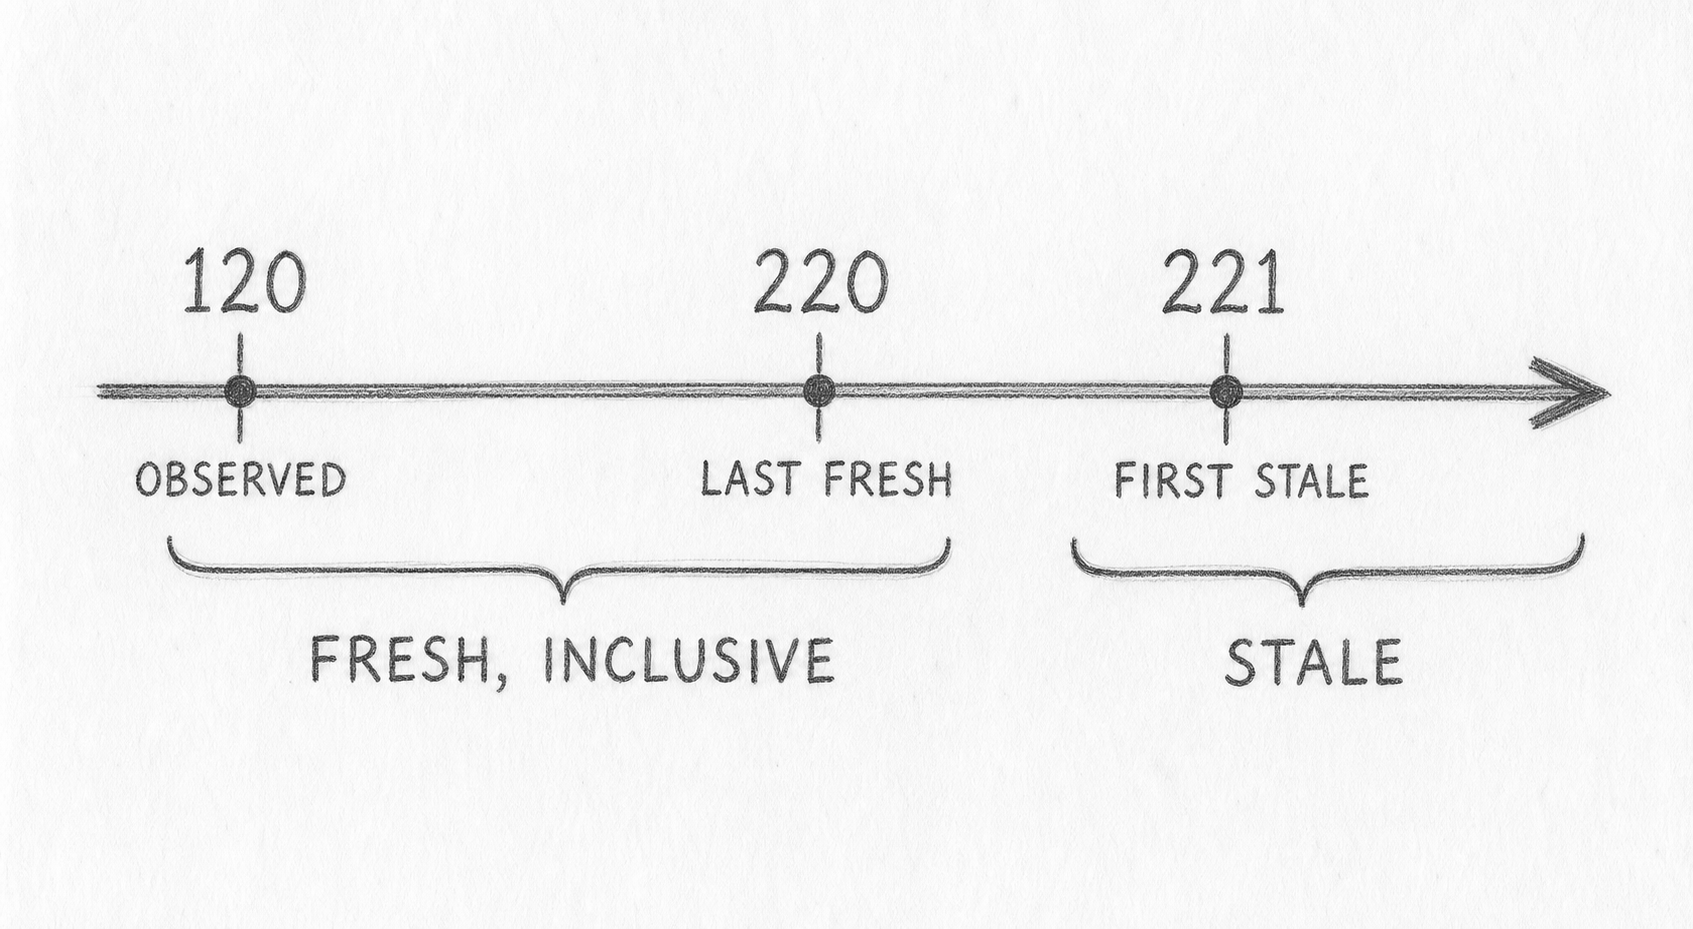
\includegraphics[width=0.92\linewidth,height=1.90in,keepaspectratio]
 {055-freshness-pencil.png}

\small\textit{Alternative text: a rough pencil timeline marks observation at
120, the inclusive last-fresh point at 220, and the first-stale point at 221.}
\end{center}

\section{Read the canonical code path}
The full sketch remains downloadable and testable as text. Its high-level
flow deliberately reads as observe, decide, present:

\begin{lstlisting}[language=C++]
const ClueConstraintUpdate update =
    observeCopiedClueCards(frame);
const Status operationStatus =
    decideClueProgress(update);
presentEvidenceWallIntent(replayIndex, frame,
                          operationStatus);
\end{lstlisting}

Each frame is one copied envelope. The sketch first proves that a four-rule
cycle is rejected, then replays four-rule progress and solve, a maximum
twelve-rule solve, stale evidence, and contradictory evidence. It changes
from the four-rule object to the twelve-rule object only at a deliberate
lifecycle boundary.

\section{Run predict, observe, interpret}
Use the canonical compile-only Mega sketch and focused host tests. Do not
credit Serial output. Before each frame, write a prediction; afterward inspect
the named memory cell or fieldwise test result.

\begin{enumerate}
 \item \textbf{Cycle fixture.} Predict
       \texttt{InvalidConfiguration}. Observe
       \texttt{cycleRejectionStatusCell} and
       \texttt{cycleRejectionDispositionCell}. Interpret success only as
       graph validation.
 \item \textbf{Four-rule progress.} Predict satisfied mask
       \texttt{0x0001}, blocked mask \texttt{0x000e}, and
       \texttt{Incomplete}. Observe \texttt{evidenceWallCells[0]}.
 \item \textbf{Four-rule solve.} Predict \texttt{0x000f},
       \texttt{0x0000}, and \texttt{Solved}. Observe cell 1.
 \item \textbf{Maximum solve.} Predict all twelve bits satisfied,
       no blocked bits, and \texttt{Solved}. Observe cell 2.
 \item \textbf{Stale frame.} Predict stale disposition and blocked
       downstream rules. Observe cell 3 and its copied clue-zero time.
 \item \textbf{Contradiction.} Predict the first five rules satisfied,
       the contradictory clue and its descendants blocked, and a
       contradiction disposition. Observe cell 4.
\end{enumerate}

\begin{tabularx}{\linewidth}{@{}l l l l X@{}}
\toprule
frame & generation & satisfied & blocked & disposition / pass\\
\midrule
progress & \blankline & \blankline & \blankline & \longblank\\[7pt]
four solved & \blankline & \blankline & \blankline & \longblank\\[7pt]
twelve solved & \blankline & \blankline & \blankline & \longblank\\[7pt]
stale & \blankline & \blankline & \blankline & \longblank\\[7pt]
contradiction & \blankline & \blankline & \blankline & \longblank\\
\bottomrule
\end{tabularx}

\section{Diagnose configuration and update faults}
\begin{center}
% ADK visual: pencil
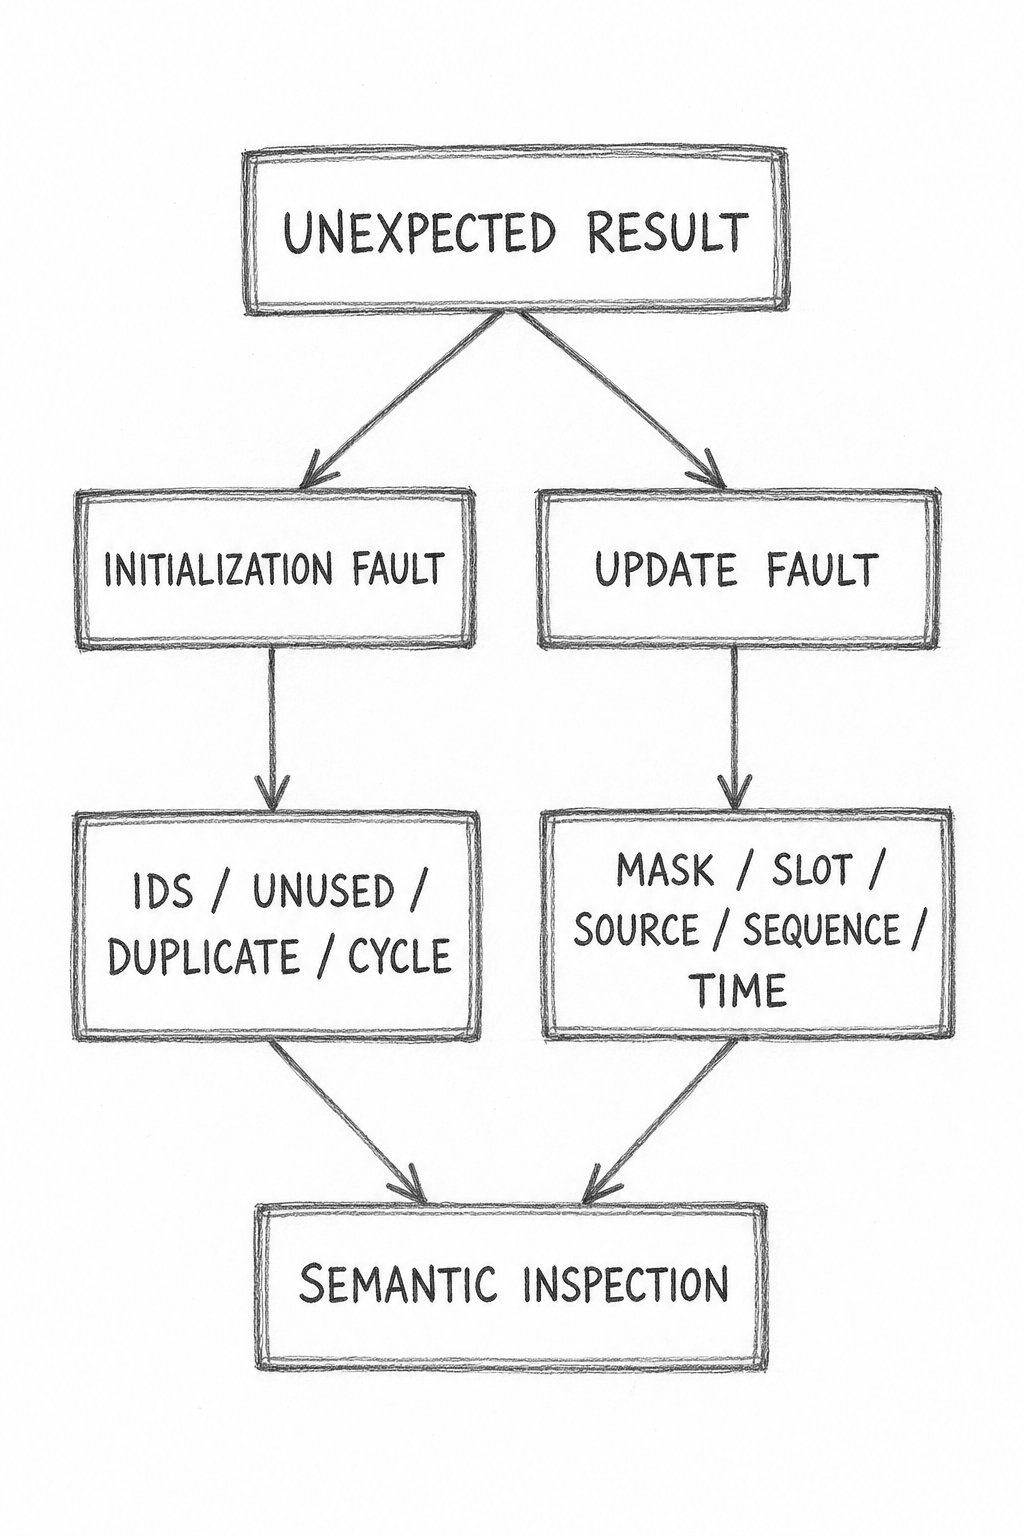
\includegraphics[width=0.70\linewidth,height=3.90in,keepaspectratio]
 {055-troubleshooting-pencil.png}

\small\textit{Alternative text: a hand-drawn troubleshooting tree separates
initialization faults in IDs, unused fields, duplicates, and cycles from
update faults in mask/slot identity, provenance, sequence, and time. Accepted
updates then lead to semantic quality, freshness, prerequisite, and term
inspection.}
\end{center}

\begin{tabularx}{\linewidth}{@{}l X X@{}}
\toprule
Symptom & Inspect first & Do not conclude\\
\midrule
initialization rejects & dense IDs, canonical unused fields, DAG & bad sensor\\
update rejects & every selected and unselected slot & partial clues were copied\\
invalid evidence & source, sequence, time, quality, status & puzzle is false\\
blocked rule & first blocking prerequisite & its own term failed\\
unsatisfied rule & first blocking term and category & input is electrically bad\\
solved & all rule snapshots and provenance & person, access, or room is safe\\
\bottomrule
\end{tabularx}

\section{Separate acquisition and safe-state evidence}
\textbf{Acquisition prediction.} A canonical configuration with 1--12 clues,
1--12 acyclic rules, valid fixed source identities, bounded age, and
canonical unused fields initializes.

\textbf{Acquisition observation.} Host tests and named memory cells inspect
initialization status, lifecycle state, configuration identity, compiled rule
results, and copied evidence. No hardware resource is acquired.

\textbf{Acquisition interpretation.} Success proves bounded configuration
and deterministic E0 policy only. It does not prove a pin, input voltage,
debounce circuit, display, storage device, latch, or Mega execution.

\textbf{Safe-state prediction and observation.} Construction, failed
initialization, reset, shutdown, invalid envelopes, and lifecycle exhaustion
cannot publish physical actuation because this component has no actuation
path. Inspect empty or inert snapshots and unchanged retained evidence where
the operation is atomic.

\textbf{Safe-state interpretation.} Software state is not an emergency stop
or power isolation. No person or animal may depend on this model for access,
confinement, egress, alarm, or life safety.

\section{Record resource evidence without overclaiming}
The promotion gates for the standalone maximum are 16/20 KiB flash,
1,536/2,048 bytes static SRAM, 384/512 bytes synchronous stack, and 512/640
bytes for the reusable object. The final canonical no-LTO Mega 2560 build
measures 8,886 bytes of flash and 1,261 bytes of static SRAM.
\texttt{sizeof(ClueConstraintModel)} is 636 bytes. Conservative
compiler-derived synchronous stack evidence is 412 bytes.

\begin{tabularx}{\linewidth}{@{}l r l X@{}}
\toprule
Evidence & Measured & Gate & Disposition\\
\midrule
flash & 8,886 B & 16/20 KiB & target and hard gate pass\\
static SRAM & 1,261 B & 1,536/2,048 B & target and hard gate pass\\
reusable object & 636 B & 512/640 B & reviewed target miss; hard gate passes\\
synchronous stack & 412 B & 384/512 B & reviewed target miss; hard gate passes\\
\bottomrule
\end{tabularx}

These values are toolchain evidence, not runtime high-water measurement or
physical verification. A target miss requires review; a hard-ceiling miss
stops promotion. The object and stack target misses were reviewed and retained
because both hard ceilings pass; they do not authorize growth past those
ceilings. Re-measure after any source, LTO setting, flags, compiler, core,
fixture, or composition change. For a local reproduction, record:
\texttt{flash} \blankline, \texttt{SRAM} \blankline,
\texttt{object} \blankline, and \texttt{stack} \blankline.

\section{Keep E1 and E2 closed}
Lesson 055 is E0. There is deliberately no wiring table, formal schematic, or
bench circuit. E1 would require exact passive input and presentation
specimens, primary electrical evidence, voltage and polarity limits, resource
ownership, an authoritative schematic, non-Serial observation, rollback, and
recorded bench acceptance. Powered actuation remains absent.

Any later E2 demonstration belongs to Lesson 057's separate gate and may use
only a restrained demonstration servo or inert current-limited relay/lamp
load with independent physical load-power removal. It may never attach to a
door, lock, occupied enclosure, alarm, emergency lighting, egress route, or
life-safety system.

\section{Exercises and acceptance record}
\begin{enumerate}
 \item Change one selected slot's clue ID while preserving its mask bit.
       Predict the operation status and prove the prior snapshot is unchanged.
 \item Add one cycle edge to the four-node diamond. Identify the exact
       configuration rule violated.
 \item Put a qualified observation exactly at the freshness limit, then one
       tick beyond it. Compare the rule and model dispositions.
 \item Change one source field, then change one value at the same sequence.
       Explain why both are evidence faults rather than ordinary mismatches.
 \item Construct a valid \texttt{NotEquals} term and predict its first
       blocking term for both categories.
\end{enumerate}

\begin{tabularx}{\linewidth}{@{}l X@{}}
\toprule
Record & Result\\
\midrule
cycle rejection & status \blankline\quad disposition \longblank\\
acquisition & status \blankline\quad initialized \blankline\\
maximum replay & satisfied \blankline\quad blocked \blankline\\
freshness boundary & last fresh \blankline\quad first stale \blankline\\
atomic rejection & retained generation \blankline\quad unchanged \blankline\\
safe-state result & \rule{4.5in}{0.4pt}\\
reviewer / date & \longblank\quad / \quad\longblank\\
\bottomrule
\end{tabularx}

This is a deterministic policy worksheet, not a hardware acceptance record.
Compare it with the accessible HTML reference, the canonical
\href{https://github.com/spincyc/adk/tree/main/examples/Lesson055ClueConstraintModel}
{Lesson 055 sketch}, and the focused host tests. Lesson 056 will compose
copied controls, presentation, stop, acknowledgement, and a two-slot audit
image without turning this clue result into access authority.

\end{document}
